\documentclass[pdftex,english,a4paper,10pt,twocolumn]{infocom}
\usepackage[pdftex,bookmarksnumbered,colorlinks,backref, bookmarks, breaklinks, linktocpage]{hyperref}
\usepackage[pdftex]{graphicx}
\usepackage{isolatin1}
\usepackage{anysize}
\usepackage{varioref}
\usepackage{latexsym}
\usepackage{enumerate}
\usepackage{float}
\usepackage{fancyvrb}
\usepackage{fancybox}
\usepackage{amsmath,amsthm, amsfonts, amssymb, amsxtra,amsopn}
\usepackage{rotating}
\usepackage{subfigure}
\usepackage{tabularx}
\usepackage{url}
\usepackage{times}
\pdfcompresslevel=9
\title{Article Test Document Title}
\author{Ramon Casellas}
\begin{document}

\maketitle

% --------------------------------------------
% Abstract 
% --------------------------------------------
\begin{abstract}

This article is just a test. This article is just a test. 
This article is just a test. This article is just a test. 
This article is just a test. This article is just a test. 
This article is just a test. This article is just a test. 
This article is just a test. This article is just a test. 
This article is just a test. This article is just a test. 
This article is just a test. This article is just a test. 
This article is just a test. This article is just a test. 
This article is just a test. This article is just a test. 
This article is just a test. This article is just a test. 
This article is just a test. This article is just a test. 
This article is just a test. This article is just a test. 
This article is just a test. This article is just a test. 
This article is just a test. This article is just a test. 
This article is just a test. This article is just a test. 
This article is just a test. This article is just a test. 
This article is just a test. This article is just a test. 
This article is just a test. This article is just a test. 
This article is just a test. This article is just a test. 
This article is just a test. This article is just a test. 

\end{abstract}



This is a `short quote'.
This is a `Quotation with a `nested quotation
containing a `nested quotation and another `nested
quotation''''.


\begin{Verbatim}[,fontfamily=default]
This is a literal layout
  It'll be a <pre> until the chunk.pl
script    fixes   things    up.
\end{Verbatim}

This article is just a test. This article is just a test.
This article is just a test. This article is just a test. 
This article is just a test. This article is just a test. 
This article is just a test. This article is just a test. 
This article is just a test. This article is just a test. 


% figure ------------------------------------------------------
\begin{figure}[hbt]
\begin{center}%
\hypertarget{testfig}{}%

\begin{Verbatim}[]
This is a
  ProgramListing

\end{Verbatim}
\caption{{{Test Figure}}}
\label{testfig}
\end{center}
\end{figure}


This para contains an xref to a figure: \hyperlink{testfig}{Figure {\ref*{testfig}}}.


% figure ------------------------------------------------------
\begin{figure}[hbt]
\begin{center}%
\hypertarget{testfig2}{}%

\begin{Verbatim}[]
A Second
  Test Figure

\end{Verbatim}
\caption{{{Test Figure2}}}
\label{testfig2}
\end{center}
\end{figure}


This para contains an \hyperlink{testfig2}{link} to a figure.
\begin{itemize}

	\item 

        \href{http://www.somewhere.com/asp?php_jsp-&fcksup?}{http://www.somewhere.com/asp?php\_jsp-\&fcksup}
      


	\item 

        \href{http://wwww.aaaaaaaa.bbbbbb.c.d.fr/aaa/bbb/ccc/ddd/eee/fff/ggg}{AAABBBCCCDDD}
        \url{http://wwww.aaaaaaaa.bbbbbb.c.d.fr/aaa/bbb/ccc/ddd/eee/fff/ggg}
      

\end{itemize}
\begin{itemize}

	\item 
Test item.


	\item 
Test item.


	\item 
Test item.

\end{itemize}
\begin{enumerate}
	\item 
Test item.


	\item 
Test item.


	\item 
Test item.


	\end{enumerate}

    
This article is just a test. This article is just a test.
This article is just a test. This article is just a test. 
This article is just a test. This article is just a test. 
This article is just a test. This article is just a test. 
This article is just a test. This article is just a test. 
This article is just a test. This article is just a test. 
This article is just a test. This article is just a test. 
This article is just a test. This article is just a test. 
This article is just a test. This article is just a test. 
This article is just a test. This article is just a test. 
This article is just a test. This article is just a test. 
This article is just a test. This article is just a test. 
This article is just a test. This article is just a test. 
This article is just a test. This article is just a test. 
This article is just a test. This article is just a test. 
This article is just a test. This article is just a test. 
This article is just a test. This article is just a test. 
This article is just a test. This article is just a test. 
This article is just a test. This article is just a test. 
This article is just a test. This article is just a test. 


% figure ------------------------------------------------------
\begin{figure}[hbt]
\begin{center}%
\hypertarget{fig}{}%

{{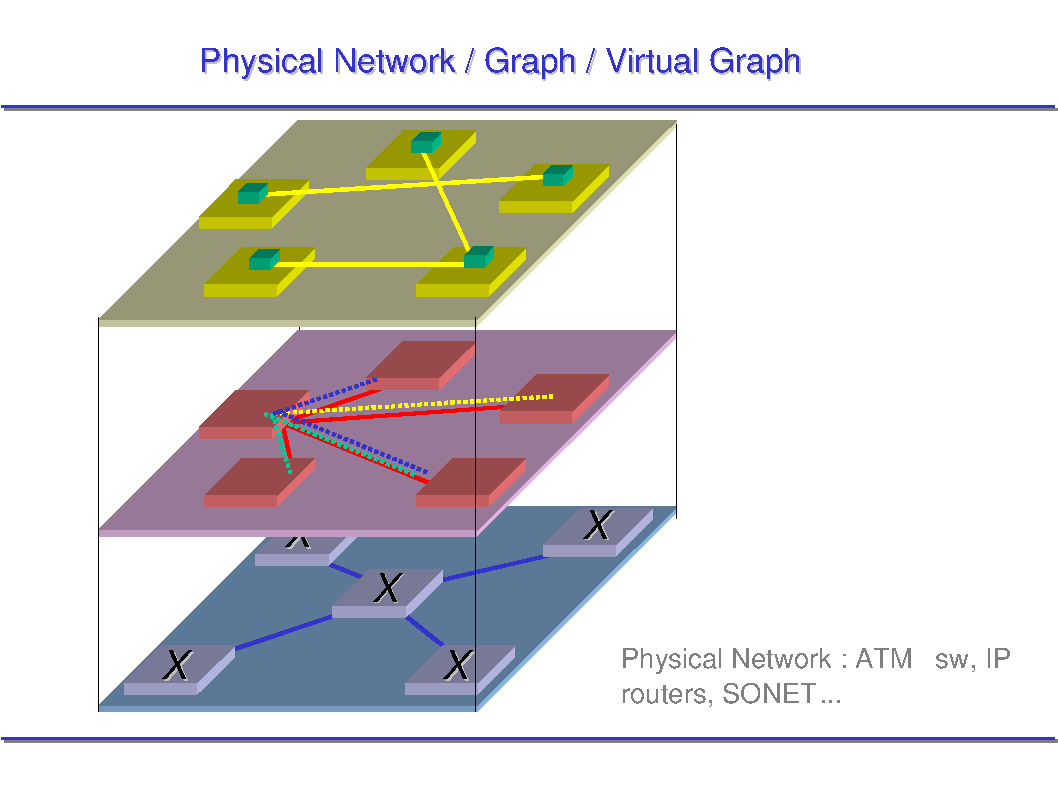
\includegraphics[scale=.50]{figures/sample}}}
\caption{{{A pdf/eps fig }}}
\label{fig}
\end{center}
\end{figure}


% ------------------------   
% Section 
\section{Lists, of course}
\label{id2719356}\hypertarget{id2719356}{}%

\begin{tabular*}{\linewidth}{ll} 
IBM's Java performance research & 
        \href{http://www.somewhere.com/asp?php_jsp-&fcksup?}{http://www.somewhere.com/asp?php\_jsp-\&fcksup}
        \\
C vs. Java speed comparisons  & 
        \url{http://www.aceshardware.com/Spades/read.php?article_id=153}
        \\
Java versus C++ & 
        \url{http://www.multimania.com/lefevre/java/ceaxx.html}
        \\
Java Performance & 
        \url{http://hepunx.rl.ac.uk/hep2java/meeting/16-03-2000/hoschek2/sld001.htm}
        \\
 
	  Java Grande Forum & 
        \url{http://www.javagrande.org/}
        \\
 
	   Java for Scientific Computing & 
        \url{http://www.npac.syr.edu/projects/javaforcse/}
        \\
 
	  The Java HotSpot Performance Engine Architecture & 
        \url{ http://java.sun.com/products/hotspot/whitepaper.html}
        \\
\end{tabular*}

{\bf No operator overloading} 
 For non-primitive types, operator can't be overloaded.
	There are attractions in allowing operator overloading to
	support mathematical operations where the notation is close to
	the normal mathematical formalism and one can take advantage of
	the operator precedence rules.
      



{\bf No automatic type narrowing.} 
 The
	type conversion which could lead to a loss of precision
	doesn't happen automatically, but variables must be cast
	explicitly. This protects the developer from certain
	hard-to-find bugs and makes the behaviour of the code
	explicit, but some may find it annoying.




% ------------------------   
% Section 
\section{First level section}
\label{id2719526}\hypertarget{id2719526}{}%

\subsection{Second level section}
\label{id2719533}\hypertarget{id2719533}{}%

\subsubsection{Section}
\label{id2719540}\hypertarget{id2719540}{}%

\newcommand{\dbappendix}[1]{\section{#1}}%
% ------------------------------------------------------------- 
% Appendixes start here
% -------------------------------------------------------------
\appendix

% -------------------------------------------------------------
% appendix:  Appendix 
% ------------------------------------------------------------- 	
\dbappendix{Appendix}
\label{id2719555}\hypertarget{id2719555}{}%

This is just a test.

This article is just a test. This article is just a test.
This article is just a test. This article is just a test. 
This article is just a test. This article is just a test. 
This article is just a test. This article is just a test. 
This article is just a test. This article is just a test. 


This article is just a test. This article is just a test.
This article is just a test. This article is just a test. 
This article is just a test. This article is just a test. 
This article is just a test. This article is just a test. 
This article is just a test. This article is just a test. 


This article is just a test. This article is just a test.
This article is just a test. This article is just a test. 
This article is just a test. This article is just a test. 
This article is just a test. This article is just a test. 
This article is just a test. This article is just a test. 


This article is just a test. This article is just a test.
This article is just a test. This article is just a test. 
This article is just a test. This article is just a test. 
This article is just a test. This article is just a test. 
This article is just a test. This article is just a test. 


This article is just a test. This article is just a test.
This article is just a test. This article is just a test. 
This article is just a test. This article is just a test. 
This article is just a test. This article is just a test. 
This article is just a test. This article is just a test. 


This article is just a test. This article is just a test.
This article is just a test. This article is just a test. 
This article is just a test. This article is just a test. 
This article is just a test. This article is just a test. 
This article is just a test. This article is just a test. 

% ------------------------------------------- 
%	
%  Bibliography
%	
% -------------------------------------------	
\bibliography{}
\begin{thebibliography}{WIDELABEL}

% -------------- biblioentry 
\bibitem[ASU96]{ASU96}
\emph{Compilers, Principles, Techniques, and Tools} , Alfred V. Aho, Ravi Sethi, and Jeffrey D. Ullman, Addison-Wesley Publishing Company, Copyright \copyright{} 1996 Bell Telephone Laboratories, Inc., 0-201-10088-6, James T. DeWolf. \label{id2719650}


% -------------- biblioentry 
\bibitem[Abbrev]{Abbrev}
\emph{A Really Full BiblioEntry} , AuthorFirstname AuthorSurname, Copyright \copyright{} 1998 Copyright holder, EditorFirstName EditorSurname, ISBN, PageNums, PubDate, PubPublisherNameAny StreetAnywhere, XX99999USA, ReleaseInfo. \label{id2719933}


% -------------- biblioentry 
\bibitem[Walsh97]{Walsh97}
\emph{} , . \label{walsh97}


\end{thebibliography}

% --------------------------------------------
% End of document
% --------------------------------------------
\end{document}
